%!TEX root = ../paper.tex

\begin{figure*}[!ht]
\centering
\noindent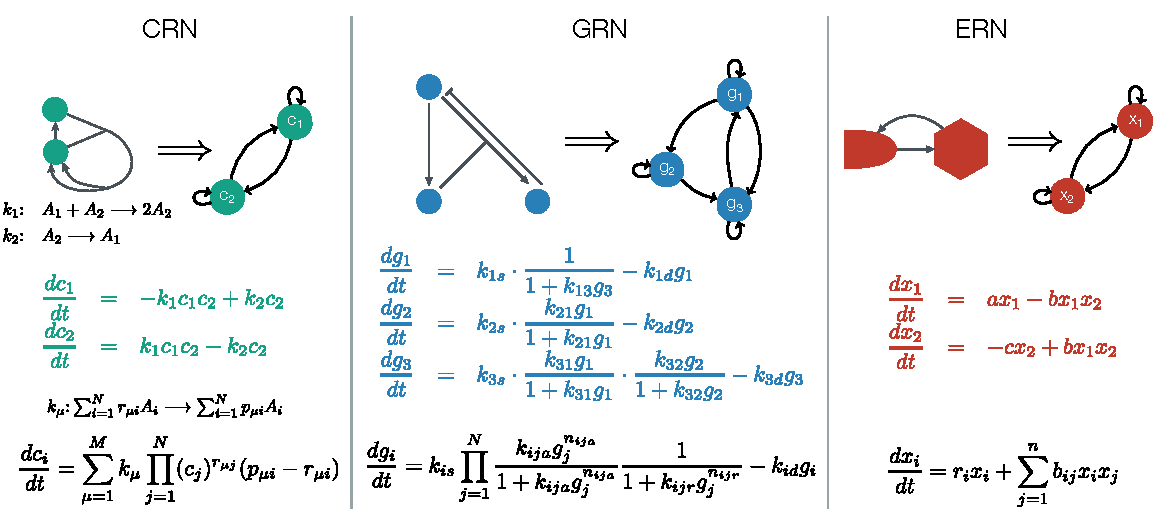
\includegraphics[width=0.8\textwidth]{fig/biomodelexamples.pdf}
\caption{{\bf Dynamical models in systems biology.} The top row represents a chemical reaction network (CRN) \cite{Shinar2010}, a gene regulatory network (GRN) \cite{Karlebach2008}, and an ecological regulatory network (ERN) \cite{Rohr2014} in terms of the graphical methods specific to each field mapped into the interaction graph, which provides a unified representation for networks across these fields. The second row represents a particular example of a system of differential equations that are used to model a biological network within each of the domains of application considered here. The third row shows the general form of a system of differential equations that can be used to model any network architecture within each domain.}
\label{fig:biomodelexamples}
\end{figure*}

\pagebreak

\begin{figure*}[!htbp]
\centering
\noindent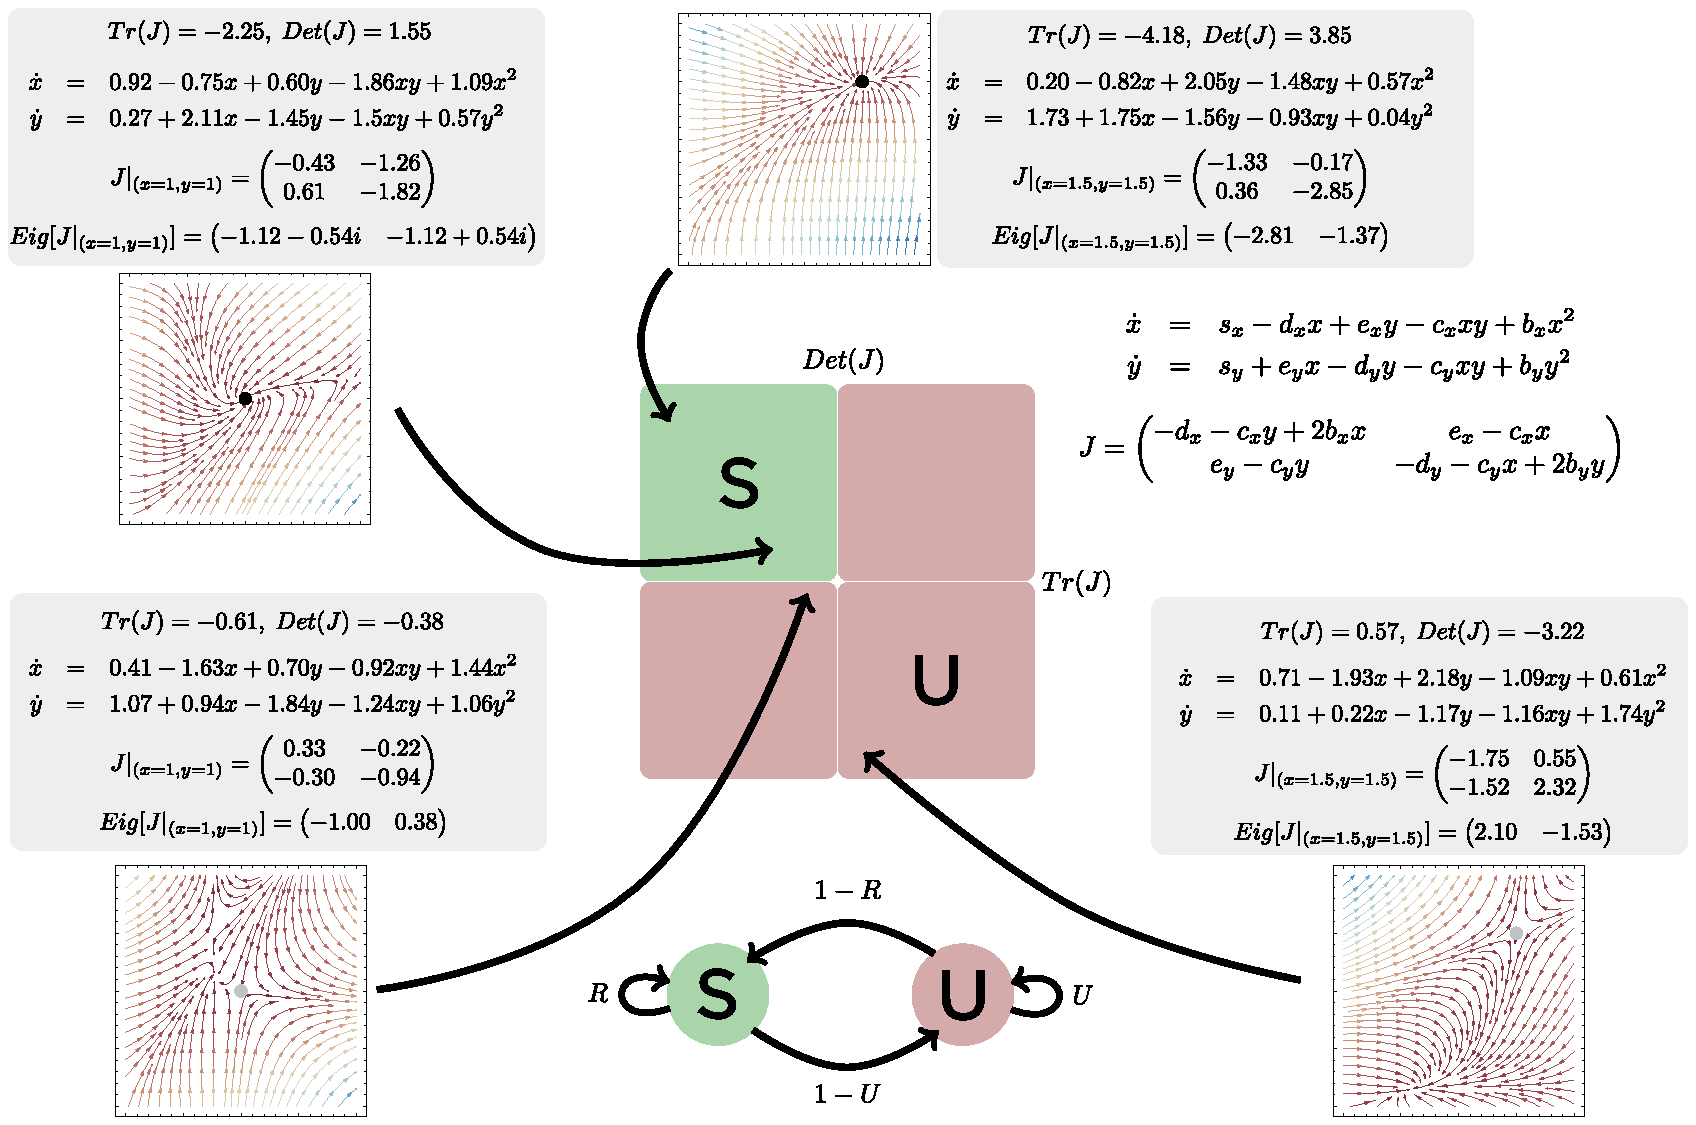
\includegraphics[width=1.0\textwidth]{fig/robustnessconcept.pdf}
\caption{{\bf Stability and robustness of biological networks.} Linearization around a steady-state of a model of a biological network allows for the assessment of the stability of that state. For two-dimensional systems, assessment of stability in terms of the trace and determinant of the Jacobian matrix associated to a particular steady-state geometrically partitions the plane into a stable region (S, blue) and an unstable region (U, red). The stochastic process induced on the stable and unstable regions that results from modifications to a given dynamical model over evolutionary timescales is represented by the state transition diagram (bottom middle). The probability of remaining in the stable region in the context of such modifications, given a previously existing stable network, is then provided by estimating $R$.}
\label{fig:robustnessconcept}
\end{figure*}

\pagebreak

\begin{figure*}[!ht]
\centering
\noindent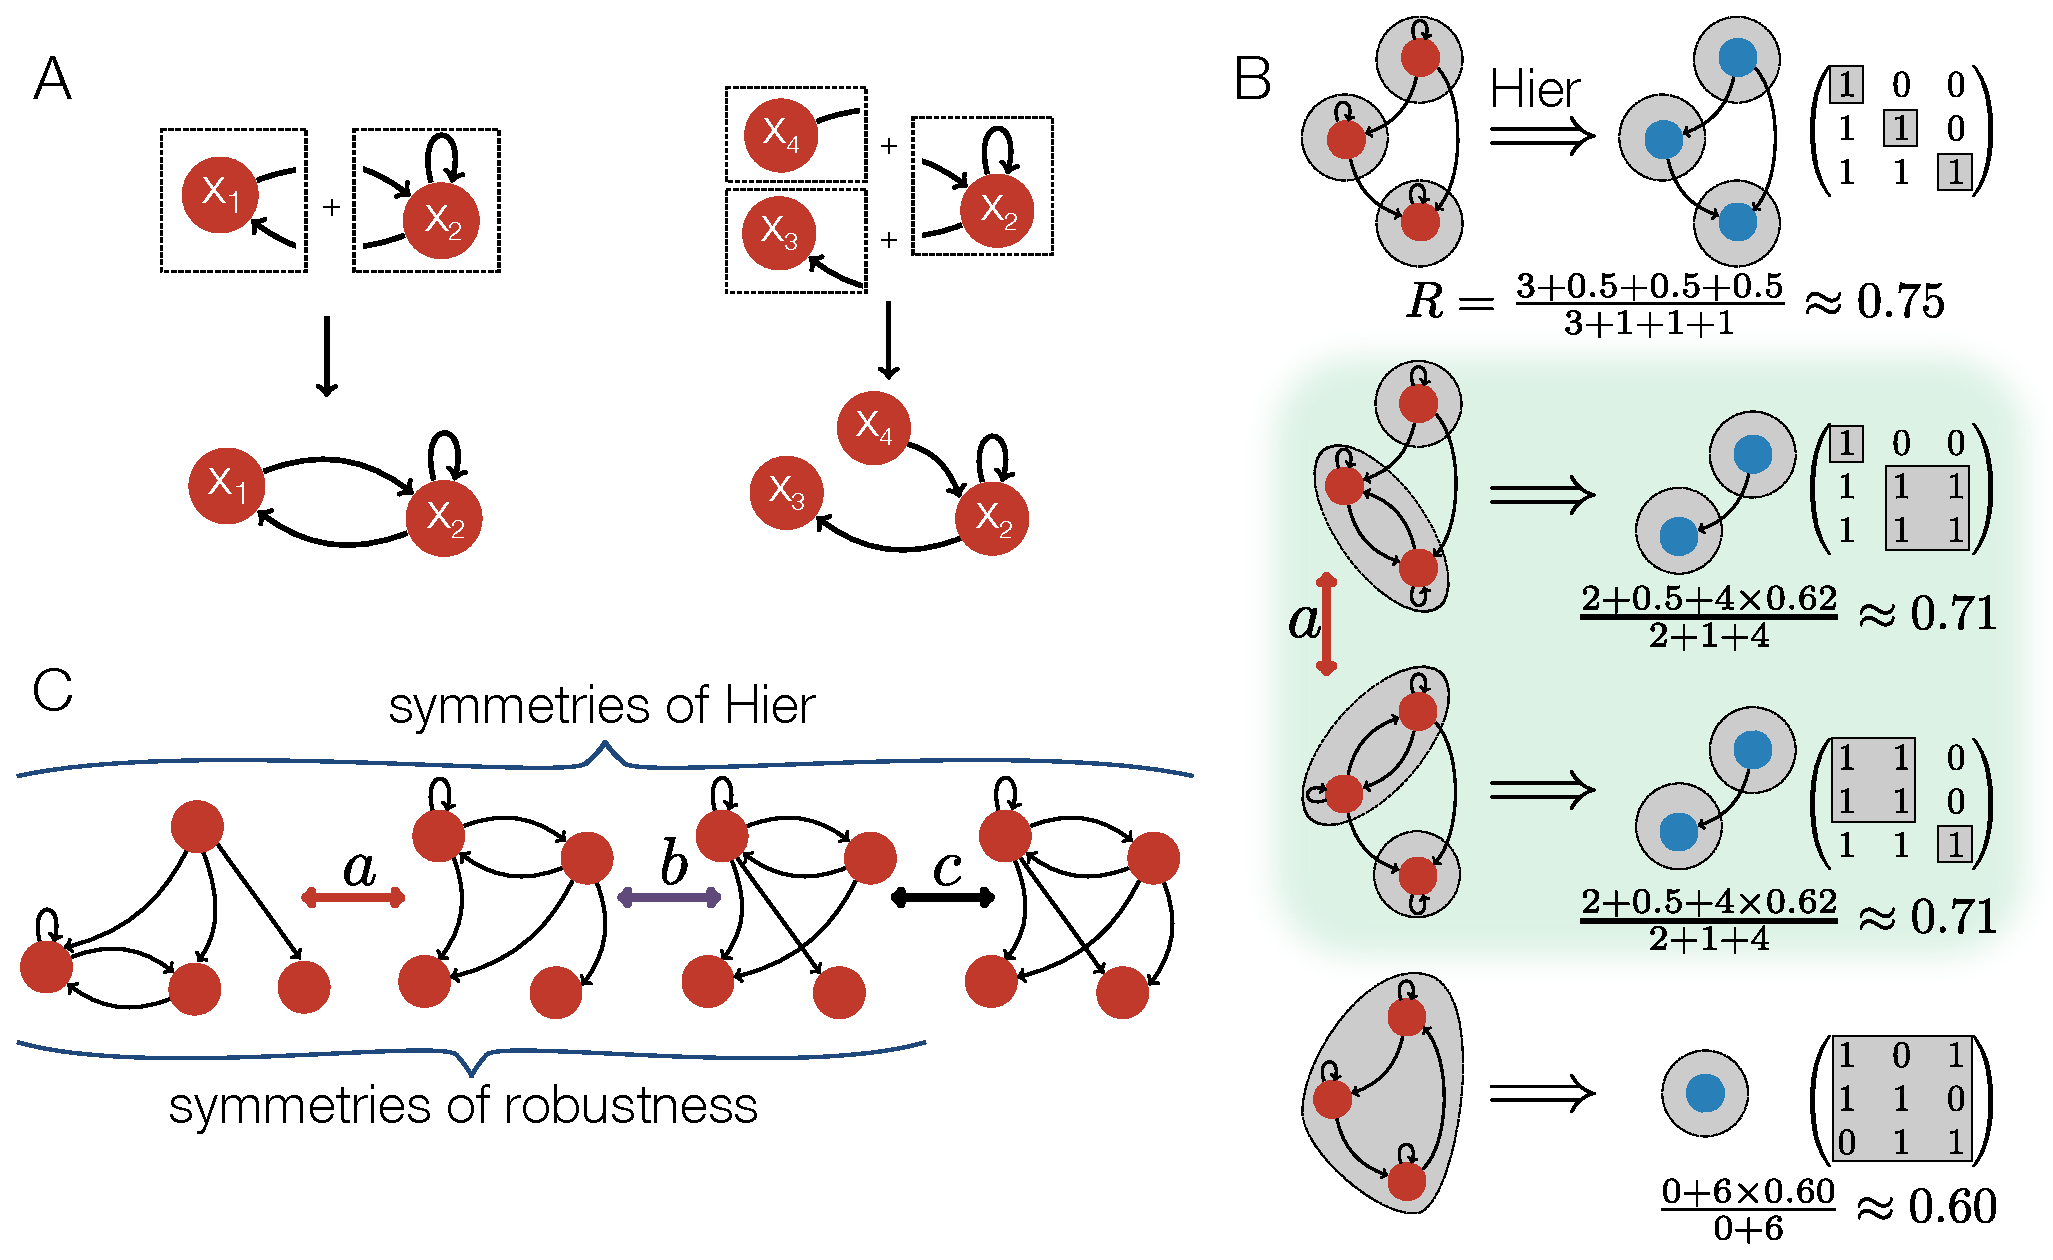
\includegraphics[width=0.8\textwidth]{fig/modsccsym.pdf}
\caption{{\bf Open systems, strongly connected components and symmetries of robustness.} (A) Example of the combination of open system modules to construct closed systems. (B) SCCs highlighted in gray for each of the four graphs representing the interdependencies relevant to four different three variable systems. The most hierarchical network, top panel, is the one that maximizes the number of SCCs and the number of links between them. We therefore define hierarchy as $max(\hbox{ED}) - \hbox{ED}$ where ED is the edit distance representing the number of link addition/deletion operations necessary to transform a given graph into the most hierarchical one. The two panels in the middle represent examples of hierarchical modular systems that posess both modularity (i.e. SCCs with more than one variable) and hierarchy. (C) Symmetries of the $\hier$ transformation between graphs and SCCs. The transformation $a$ represents an interchange of SCCs, $b$ moving a link between nodes in a component and $c$ adding a link. All three transformations represent symmetries of the $\hier$ transformation from graphs to SCCs while only $a$ and $b$ are symmetries of robustness.}
\label{fig:modsccsym}
\end{figure*}

\pagebreak

\begin{figure*}[!ht]
\centering
\noindent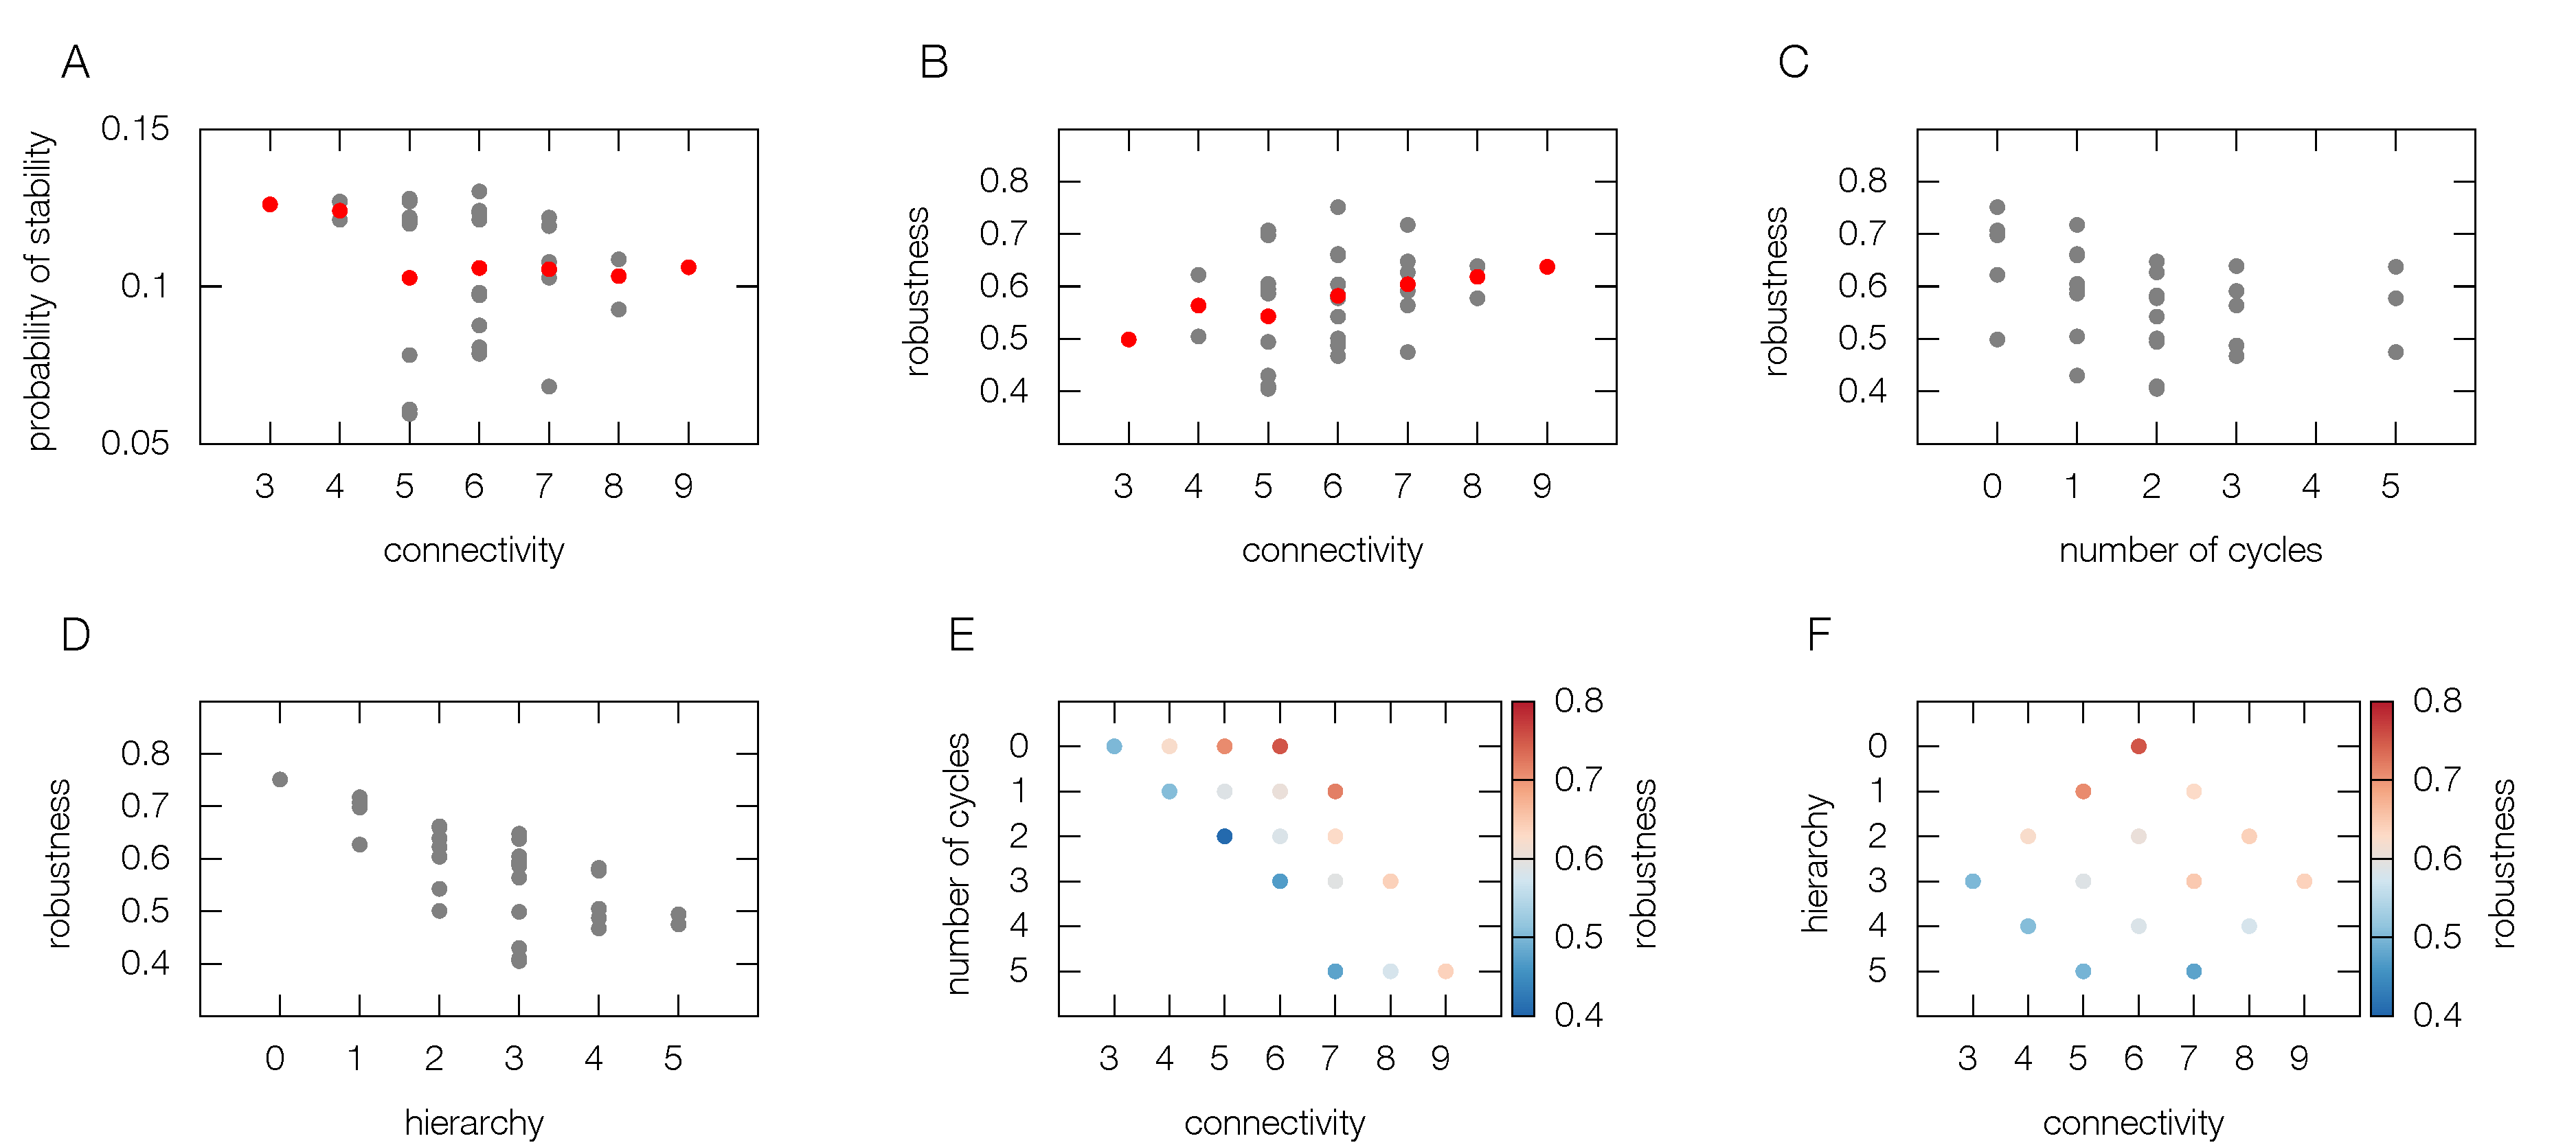
\includegraphics[width=0.8\textwidth]{fig/combinedfigs.pdf}
\caption{{\bf Characterization of stability and robustness according to properties of system structure for three variable systems} (A) Robustness versus connectivity. The red line represents a best fit in the least-squares sense with Pearson product-moment correlation coefficient $r=0.29$. The lowest and highest robustness network architectures are labelled. Other network architectures are shown in \ref{tab:structstabmat3}. (B) Robustness versus hierarchy. Correlation coefficient $r=0.67$. (C) Number of cycles and (D) hierarchy vs connectivity and robustness. The color of each point represents the average robustness of all graphs having the parameters specified on the $x$ and $y$ axes.
}
\label{fig:combined}
\end{figure*}

% \begin{figure}[!ht]
% \centering
% \noindent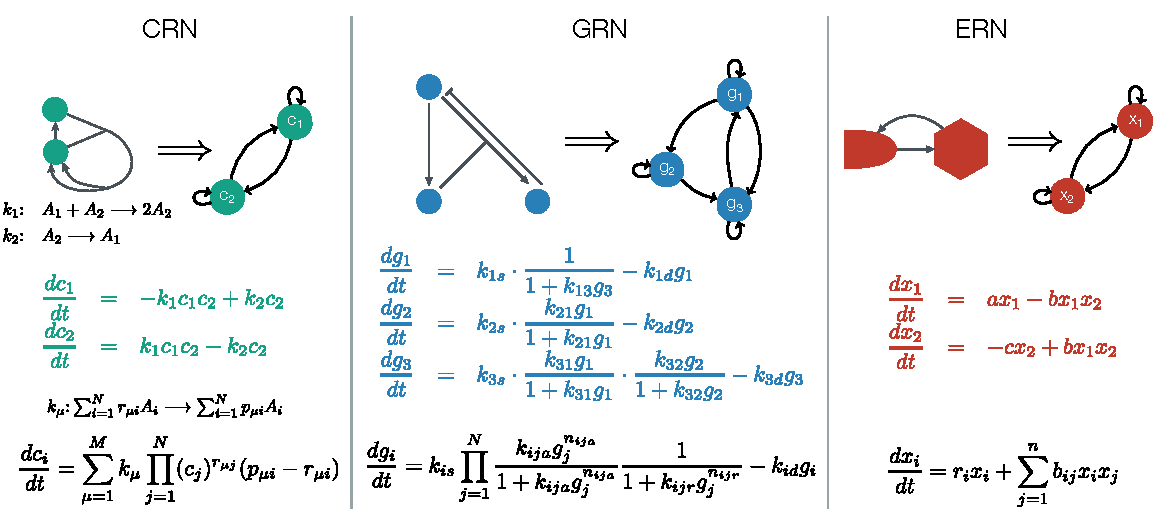
\includegraphics[width=0.9\columnwidth]{fig/biomodelexamples.pdf}
% \caption{{\bf Dynamical models in systems biology.} The top row represents a chemical reaction network (CRN) \cite{Shinar2010}, a gene regulatory network (GRN) \cite{Karlebach2008}, and an ecological regulatory network (ERN) \cite{Rohr2014} in terms of the graphical methods specific to each field mapped into the interaction graph, which provides a unified representation for networks across these fields. The second row represents a particular example of a system of differential equations that are used to model a biological network within each of the domains of application considered here. The third row shows the general form of a system of differential equations that can be used to model any network architecture within each domain.}
% \label{fig:biomodelexamples}
% \end{figure}

% \pagebreak

% \begin{figure}[!ht]
% \centering
% \noindent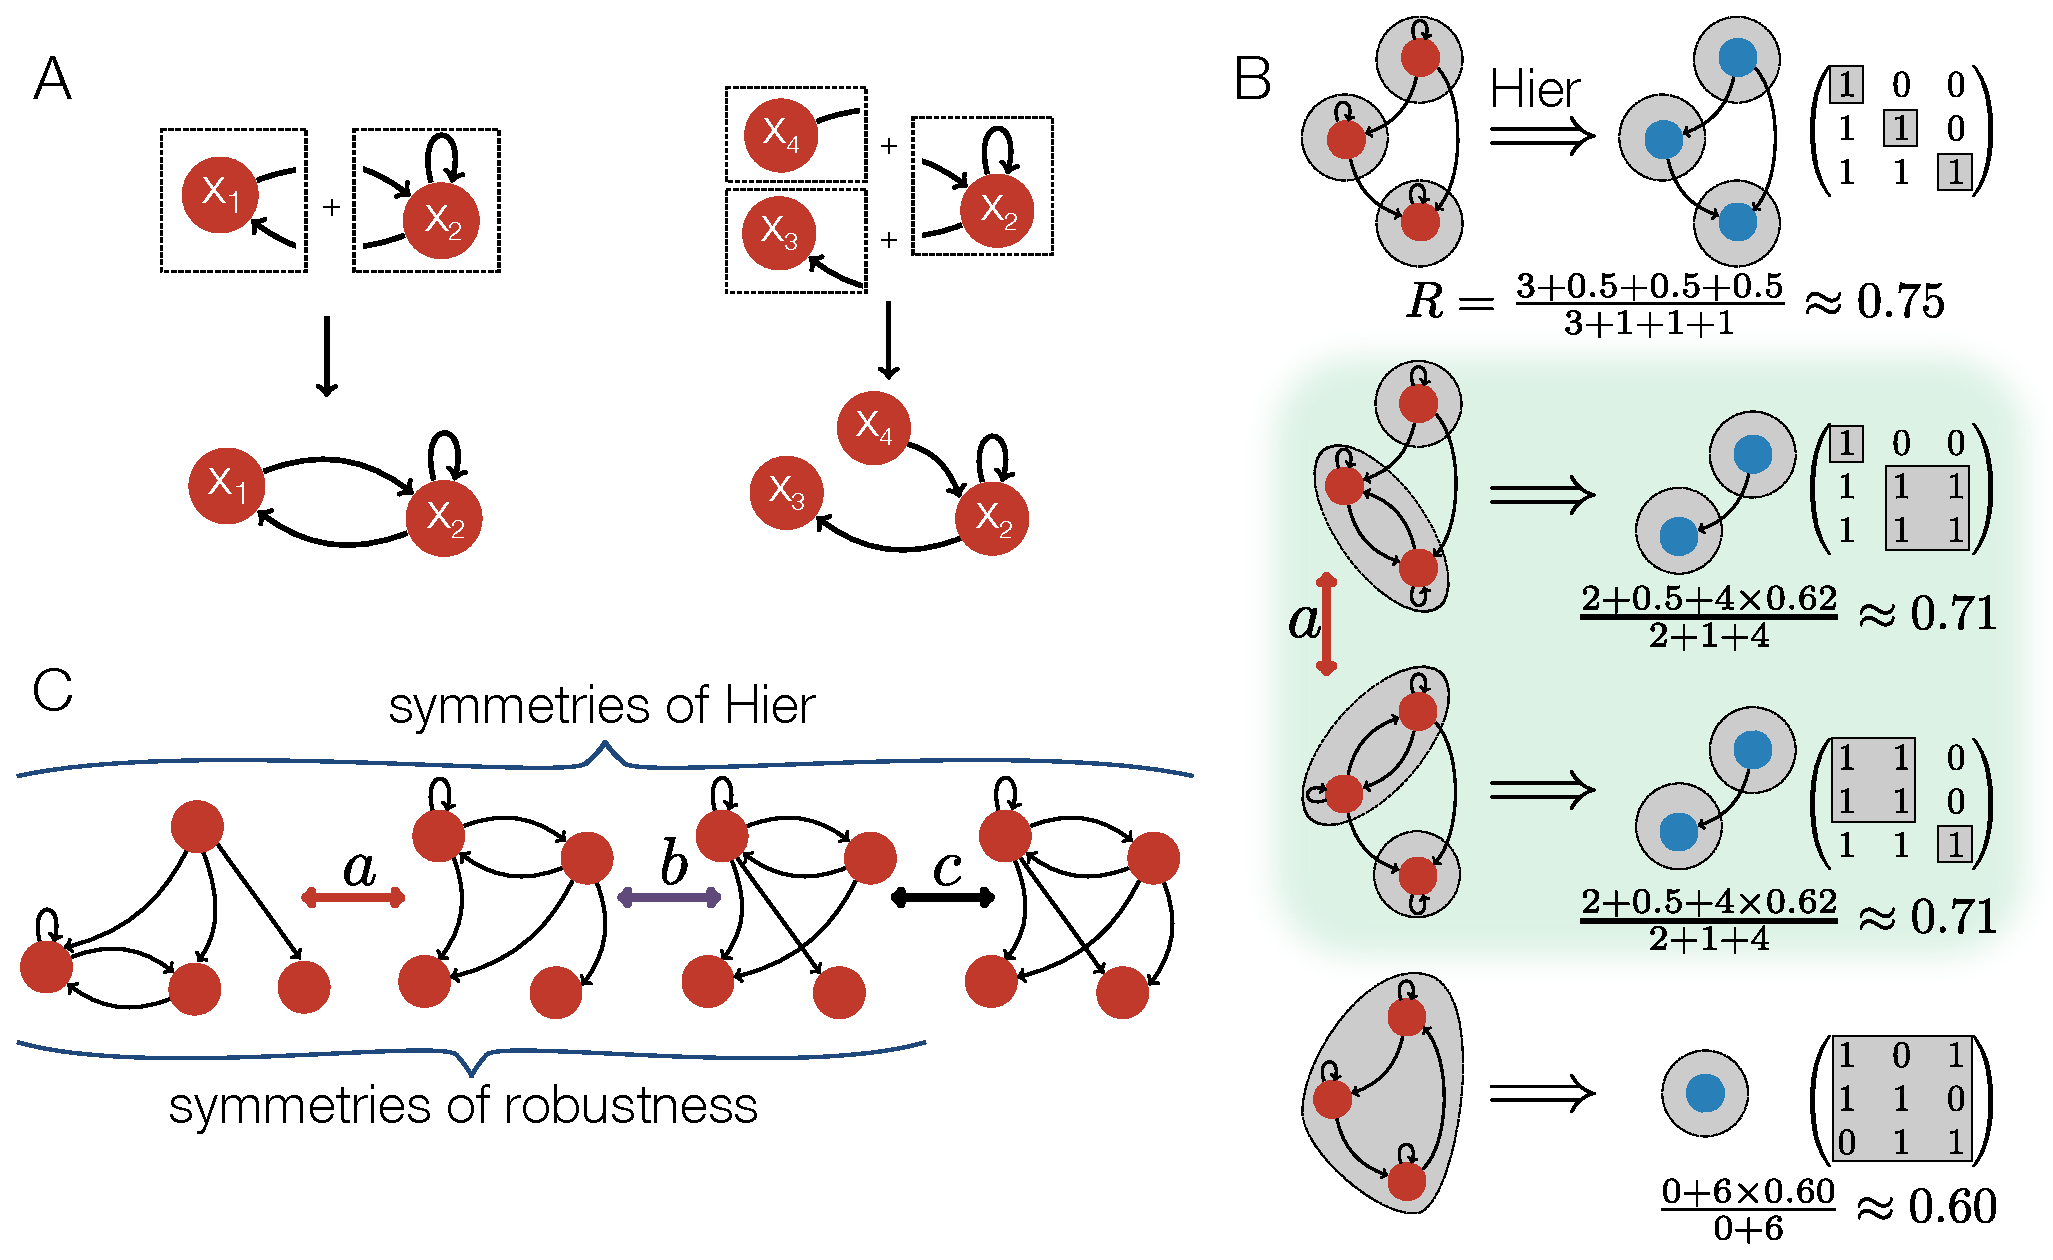
\includegraphics[width=0.9\columnwidth]{fig/modsccsym.pdf}
% \caption{{\bf Open systems, strongly connected components and symmetries of robustness.} (A) Example of the combination of open system modules to construct closed systems. (B) SCCs highlighted in gray for each of the four graphs representing the interdependencies relevant to four different three variable systems. The most hierarchical network, top panel, is the one that maximizes the number of SCCs and the number of links between them. We therefore define hierarchy as $max(\hbox{ED}) - \hbox{ED}$ where ED is the edit distance representing the number of link addition/deletion operations necessary to transform a given graph into the most hierarchical one. The two panels in the middle represent examples of hierarchical modular systems that posess both modularity (i.e. SCCs with more than one variable) and hierarchy. (C) Symmetries of the $\hier$ transformation between graphs and SCCs. The transformation $a$ represents an interchange of SCCs, $b$ moving a link between nodes in a component and $c$ adding a link. All three transformations represent symmetries of the $\hier$ transformation from graphs to SCCs while only $a$ and $b$ are symmetries of robustness.}
% \label{fig:modsccsym}
% \end{figure}

% \pagebreak


% \begin{figure}[!ht]
% \centering
% \noindent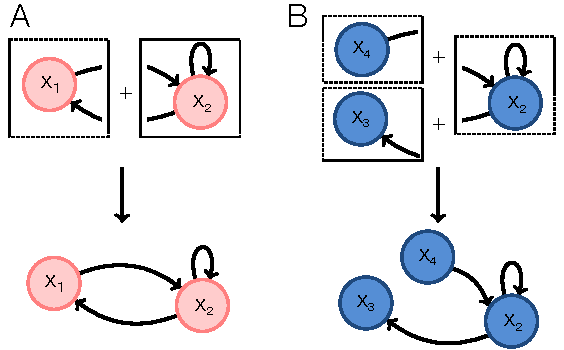
\includegraphics[width=0.4\columnwidth]{fig/examplesystemmodules.pdf}
% \caption{{\bf Example of the combination of open system modules to construct closed systems.} (A) Example of combining two open modules to construct a closed system of two components (B) Analogous example for combining three open modules to construct a closed system with three components}
% \label{fig:examplesystemmodules}
% \end{figure}

% \pagebreak

% \begin{figure}[!ht]
% \centering
% \noindent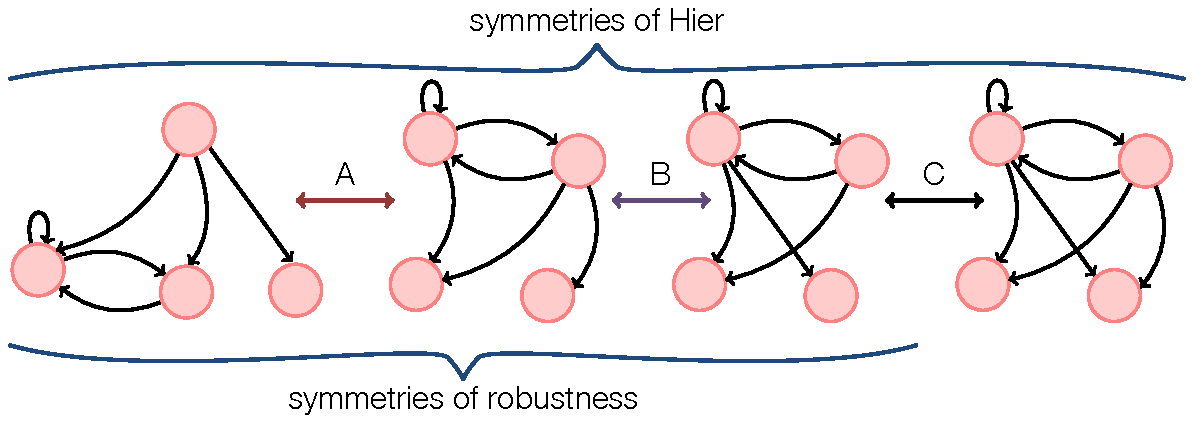
\includegraphics[width=0.7\columnwidth]{fig/hiertransformations.pdf}
% \caption{{\bf Symmetries of the $\hier$ transformation between graphs and SCCs.} The transformation A represents an interchange of SCCs, B moving a link between nodes in a component and C adding a link. All three transformations represent symmetries of the $\hier$ transformation from graphs to SCCs while only A and B are symmetries of robustness.}
% \label{fig:hiertransformations}
% \end{figure}

% \pagebreak

% \begin{figure}[!ht]
% \centering
% \noindent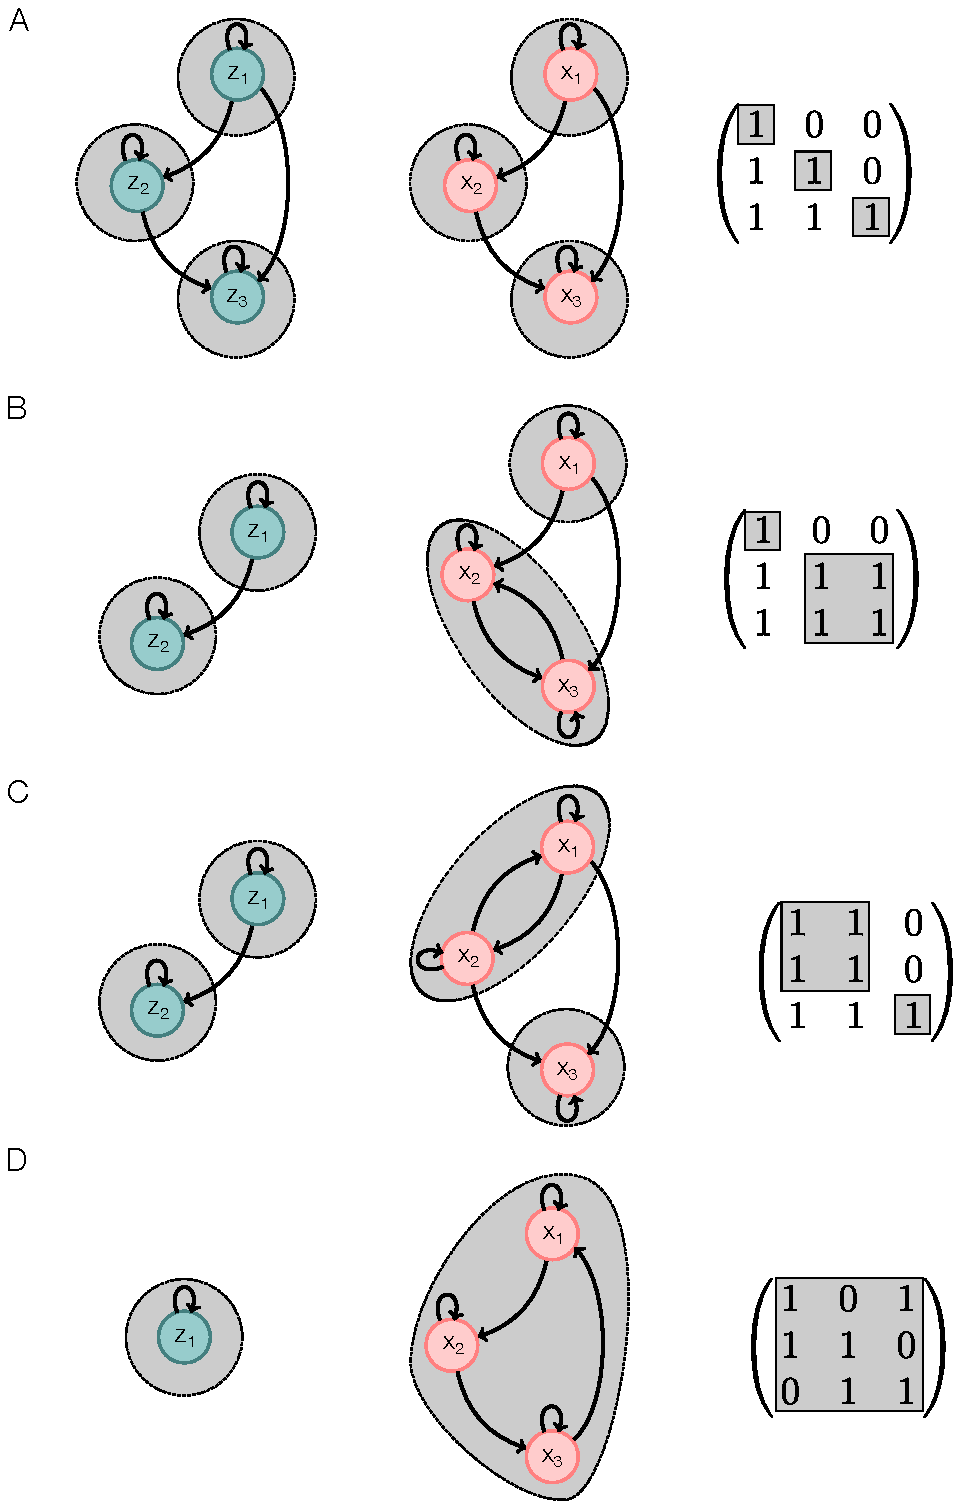
\includegraphics[width=0.4\columnwidth]{fig/scc2.pdf}
% \caption{{\bf Example of strongly connected components.} (A) - (D) show strongly connected components highlighted in gray for each of the four graphs representing the interdependencies relevant to four different three variable systems. Note that the most hierarchical system in (A) has the highest possible number of connected components, three, whereas the system containing a single cycle and therefore posessing no hierarchy contains only one connected component. Systems (B) and (C) represent examples of hierarchical modular systems that posess both modularity and hierarchy.}
% \label{fig:scc}
% \end{figure}

% \pagebreak

% \begin{figure}[!ht]
% \centering
% \noindent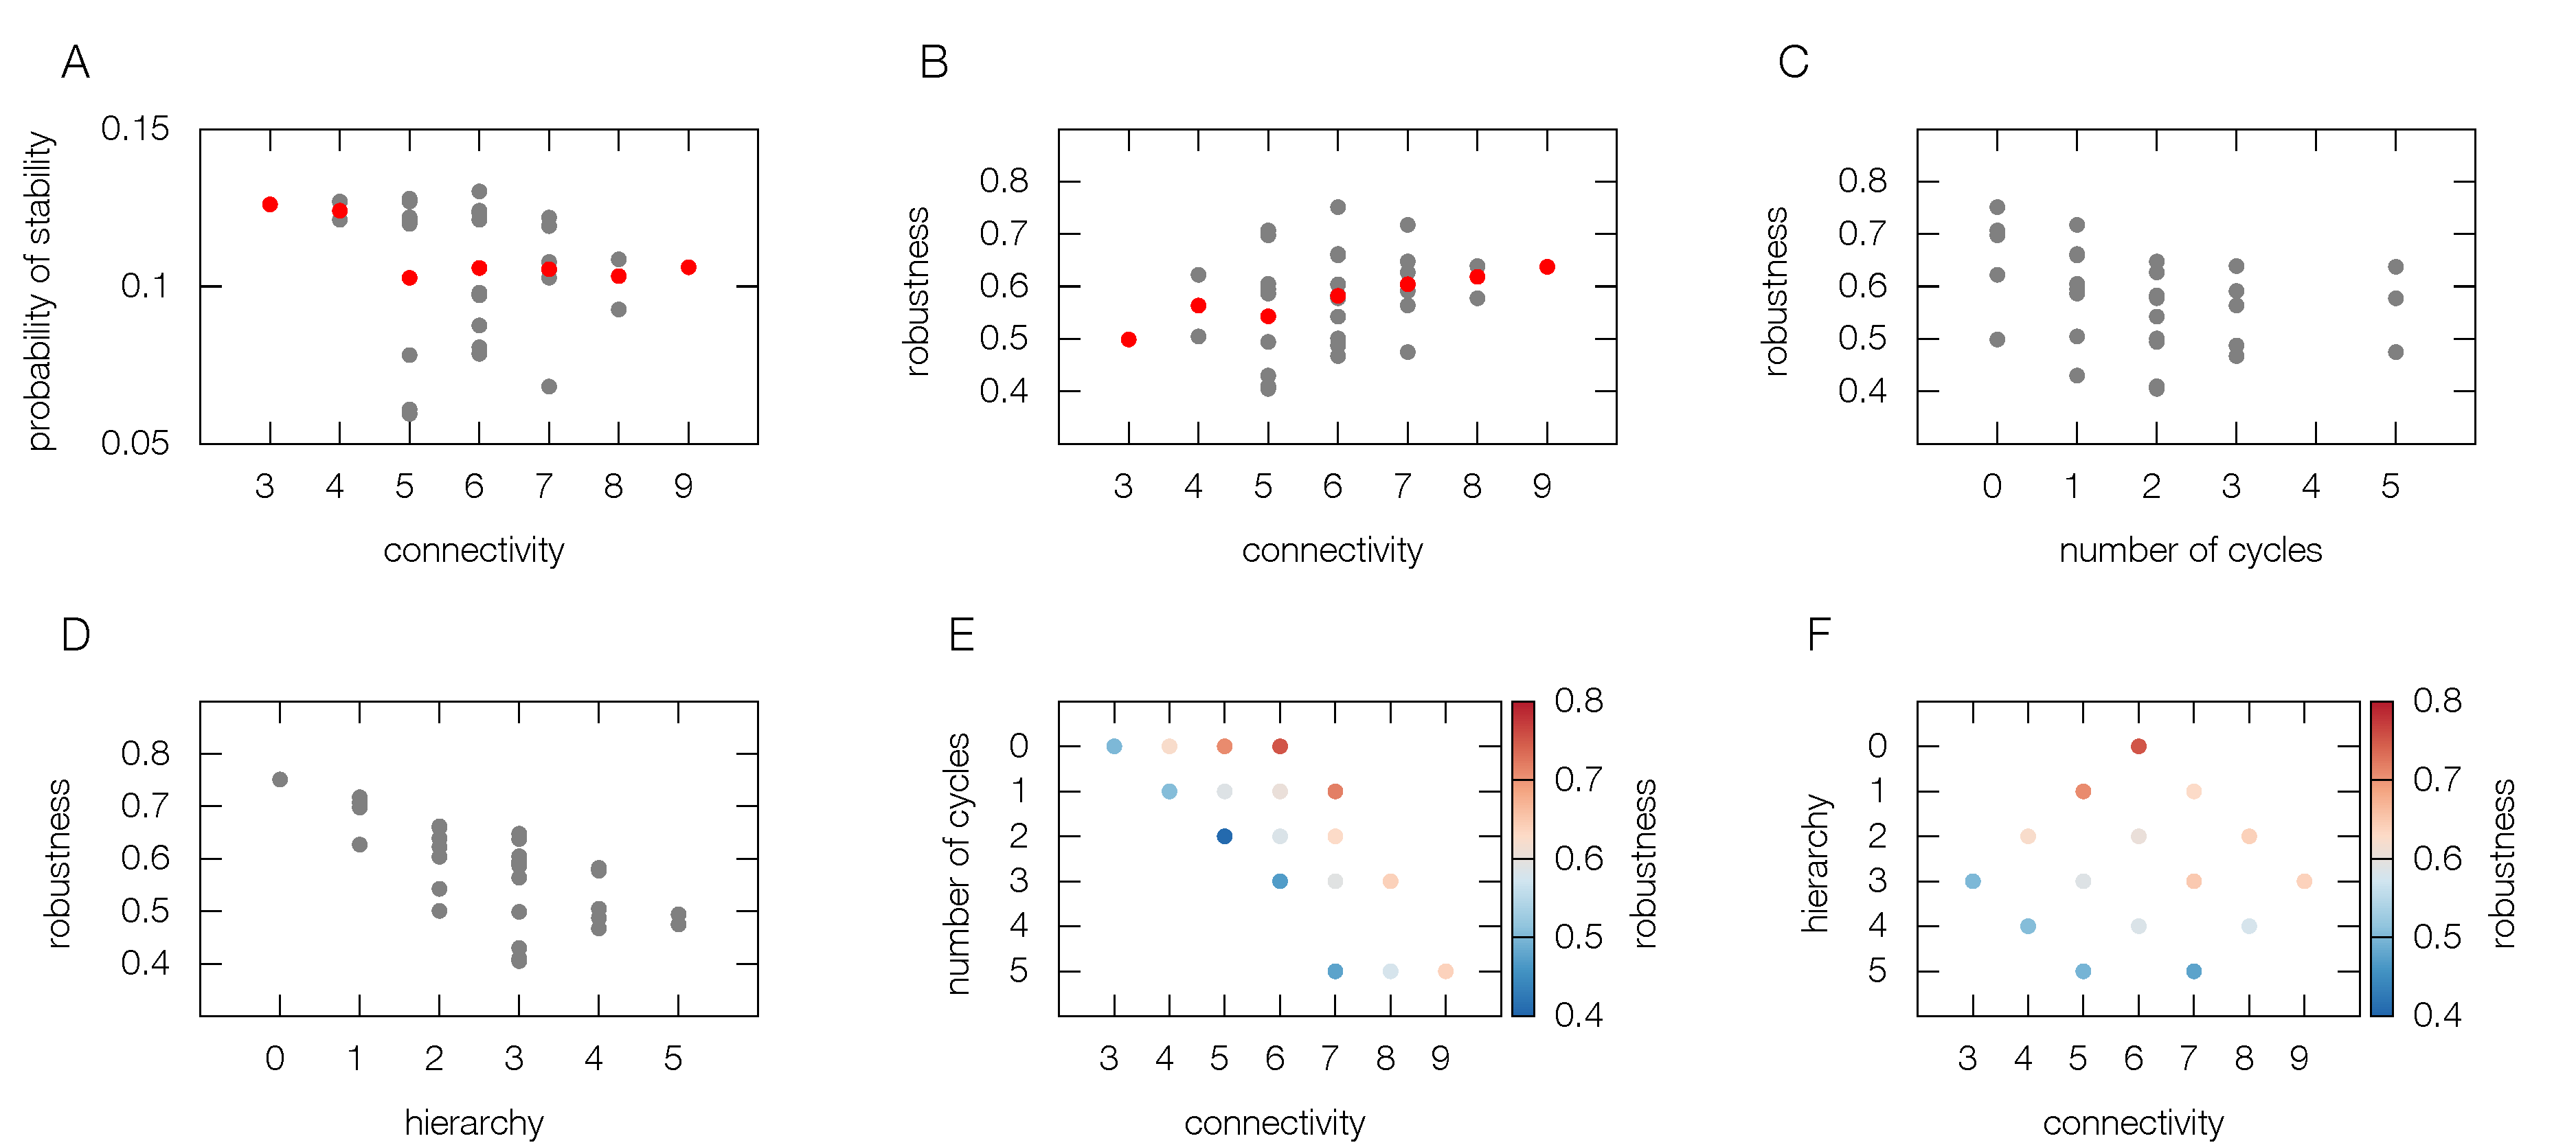
\includegraphics[width=1.0\columnwidth]{fig/combinedfigs.pdf}
% \caption{{\bf Characterization of stability and robustness according to properties of system structure for three variable systems} (A) Robustness versus connectivity. The red line represents a best fit in the least-squares sense with Pearson product-moment correlation coefficient $r=0.29$. The lowest and highest robustness network architectures are labelled. Other network architectures are shown in \ref{tab:structstabmat3}. (B) Robustness versus hierarchy. Correlation coefficient $r=0.67$. (C) Number of cycles and (D) hierarchy vs connectivity and robustness. The color of each point represents the average robustness of all graphs having the parameters specified on the $x$ and $y$ axes.
% }
% \label{fig:combined}
% \end{figure}

% \pagebreak

% \begin{figure}[!ht]
% \centering
% \noindent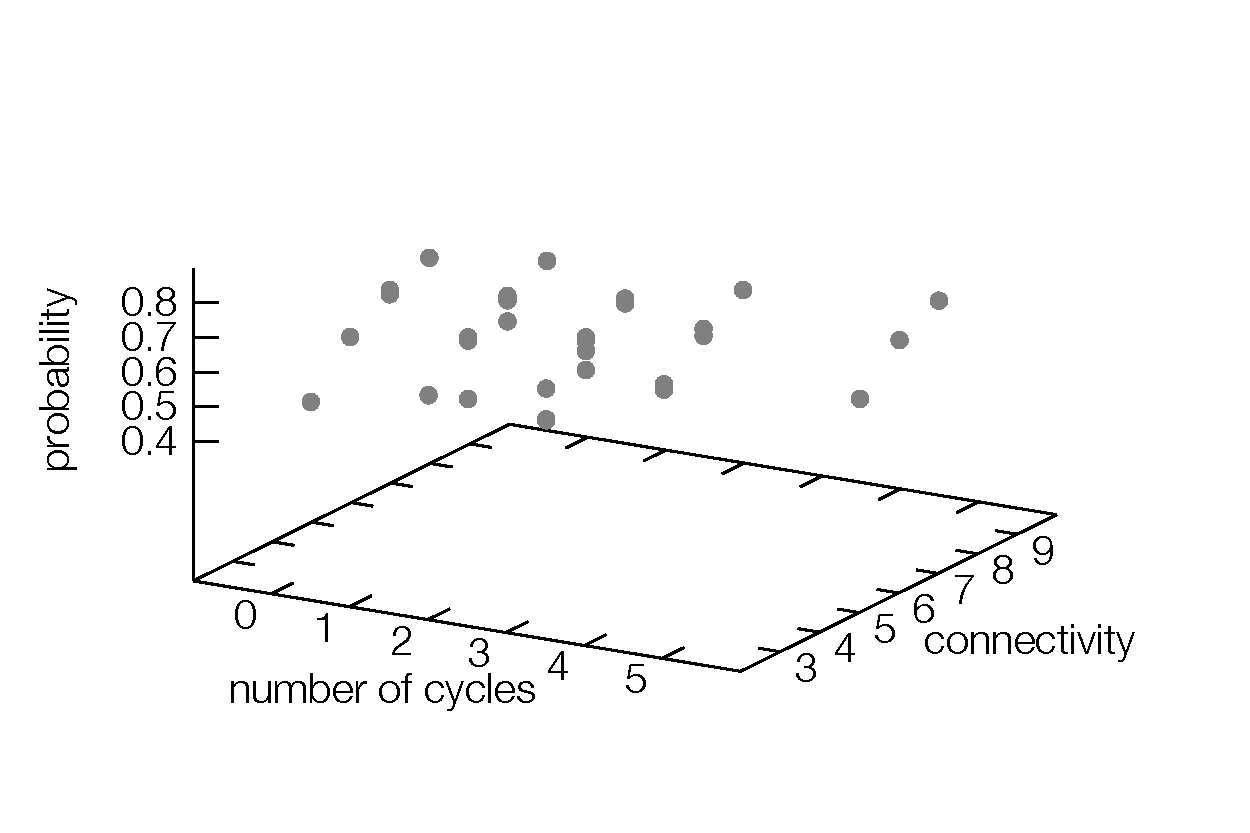
\includegraphics[width=0.8\columnwidth]{fig/connectcycle3D3x3.pdf}
% \caption{{\bf Robustness versus number of cycles and connectivity for three variable systems.} Each point represents the average robustness of all graphs having a given number of cycles and connectivity.}
% \label{fig:connectcycle3D3x3}
% \end{figure}

% \pagebreak

% \begin{figure}[!ht]
% \centering
% \noindent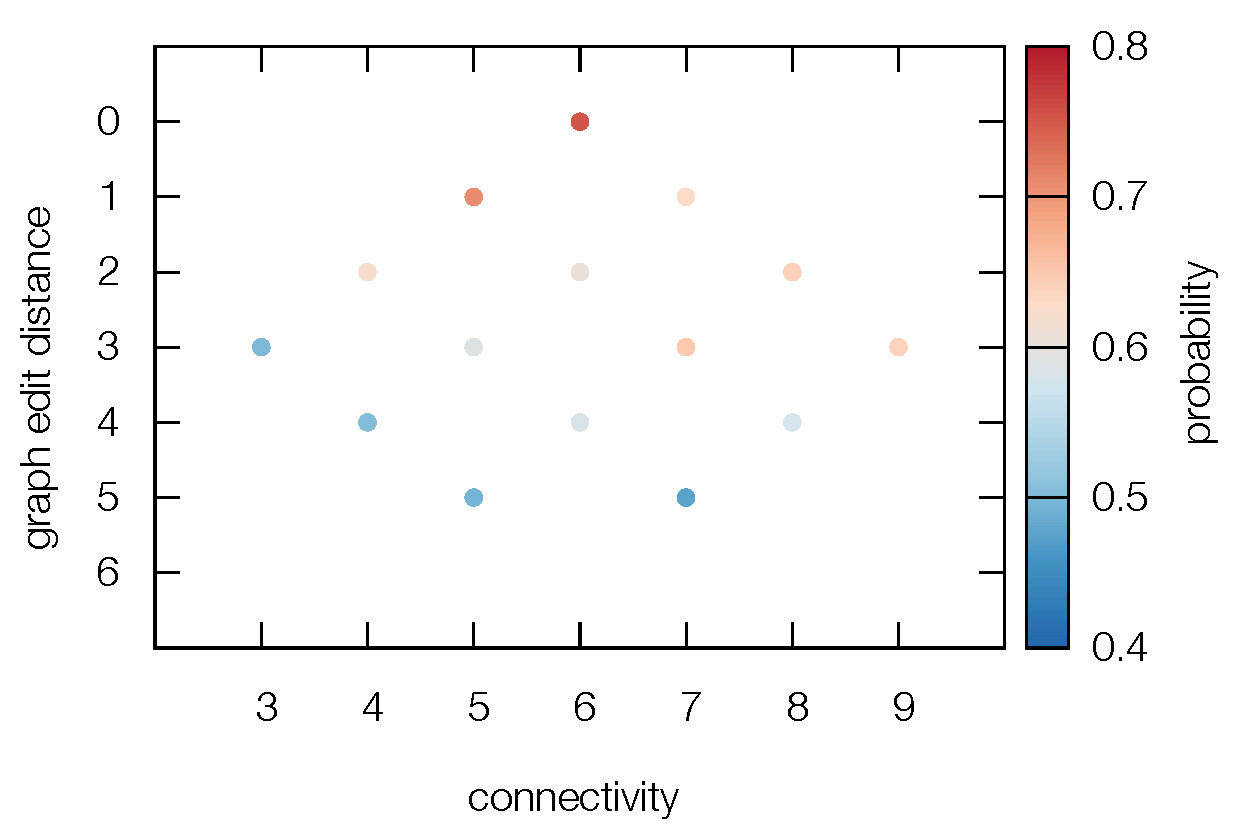
\includegraphics[width=0.8\columnwidth]{fig/connectdist3D3x3.pdf}
% \caption{{\bf Robustness versus hierarchy and connectivity for three variable systems.} Each point represents the average robustness of all graphs having a given hierarchy and connectivity.}
% \label{fig:connectdist3D3x3}
% \end{figure}

